% ch8.tex
% Dieses Werk ist unter einem Creative Commons Namensnennung-Keine kommerzielle Nutzung-Weitergabe
% unter gleichen Bedingungen 3.0 Deutschland Lizenzvertrag lizenziert. Um die Lizenz anzusehen, gehen Sie bitte
% zu http://creativecommons.org/licenses/by-nc-sa/3.0/de/ oder schicken Sie einen Brief an
% Creative Commons, 171 Second Street, Suite 300, San Francisco, California 94105, USA.


%\chapter{Turtles galore}\index{turtle!advanced}\label{ch:turtlesgalore}
\chapter{Invasion der Schildkröten}\index{Schildkröte!fortgeschrittene Funktionen}\label{ch:turtlesgalore}


%Let's get back to the \code{turtle} module we started looking at in Chapter~\ref{ch:turtles}. Remember that to setup the canvas for the turtle to draw on, we need to import the module and the create the `Pen' object:
Lass uns wieder das \code{turtle} (Schildkröte) Modul anschauen, das wir schon in Kapitel~\ref{ch:turtles} angesehen haben. Um zuerst wieder die Leinwand zu erzeugen, müssen wir das Modul importieren und dann das `Pen' Objekt erzeugen:

%\begin{Verbatim}[frame=single]
%>>> import turtle
%>>> t = turtle.Pen()
%\end{Verbatim}
\begin{Verbatim}[frame=single]
>>> import turtle
>>> schildkroete = turtle.Pen()
\end{Verbatim}

%We can now use basic functions to move the turtle around the canvas and draw simple shapes, but it's more interesting to use some of what we've already covered in the previous chapters.  For example, the code we used to create a square earlier was:
Jetzt können wir wieder mit den bekannten Funktionen die Schildkröte auf der Leinwand rumbewegen und einfache Formen zeichnen. Oder aber wir verwenden ein Paar Dinge, die wir in den letzten Kapiteln gelernt haben. Bis jetzt hat unser Code um ein Rechteck zu zeichnen so ausgesehen:

%\begin{Verbatim}[frame=single]
%>>> t.forward(50)
%>>> t.left(90)
%>>> t.forward(50)
%>>> t.left(90)
%>>> t.forward(50)
%>>> t.left(90)
%\end{Verbatim}
\begin{Verbatim}[frame=single]
>>> schildkroete.forward(50)
>>> schildkroete.left(90)
>>> schildkroete.forward(50)
>>> schildkroete.left(90)
>>> schildkroete.forward(50)
>>> schildkroete.left(90)
\end{Verbatim}

\noindent
%We can rewrite this using a for-loop:
Wenn wir das mit einer for-Schleife machen, könnte es so aussehen:

%\begin{Verbatim}[frame=single]
%>>> t.reset()
%>>> for x in range(1,5):
%...     t.forward(50)
%...     t.left(90)
%...
%\end{Verbatim}
\begin{Verbatim}[frame=single]
>>> schildkroete.reset()
>>> for x in range(1,5):
...     schildkroete.forward(50)
...     schildkroete.left(90)
...
\end{Verbatim}

%This is certainly less typing, but for something a bit more interesting, try the following:
Das ist schon viel weniger Tipparbeit und damit es interessanter aussieht probier das folgende:

%\begin{Verbatim}[frame=single]
%>>> t.reset()
%>>> for x in range(1,9):
%...     t.forward(100)
%...     t.left(225)
%...
%\end{Verbatim}
\begin{Verbatim}[frame=single]
>>> schildkroete.reset()
>>> for x in range(1,9):
...     schildkroete.forward(100)
...     schildkroete.left(225)
...
\end{Verbatim}

%This code produces the 8-point star shown in figure~\ref{fig20} (the turtle turns 225 degrees, each time it goes forward 100 pixels).
Dieser Code erzeugt einen 8-zackigen Stern wie in Abbildung~\ref{fig20} (die Schildkröte dreht sich immer um 225 Grad, jedes mal wenn sie um 100 Pixel zurückgelegt hat).

\begin{figure}
\begin{center}
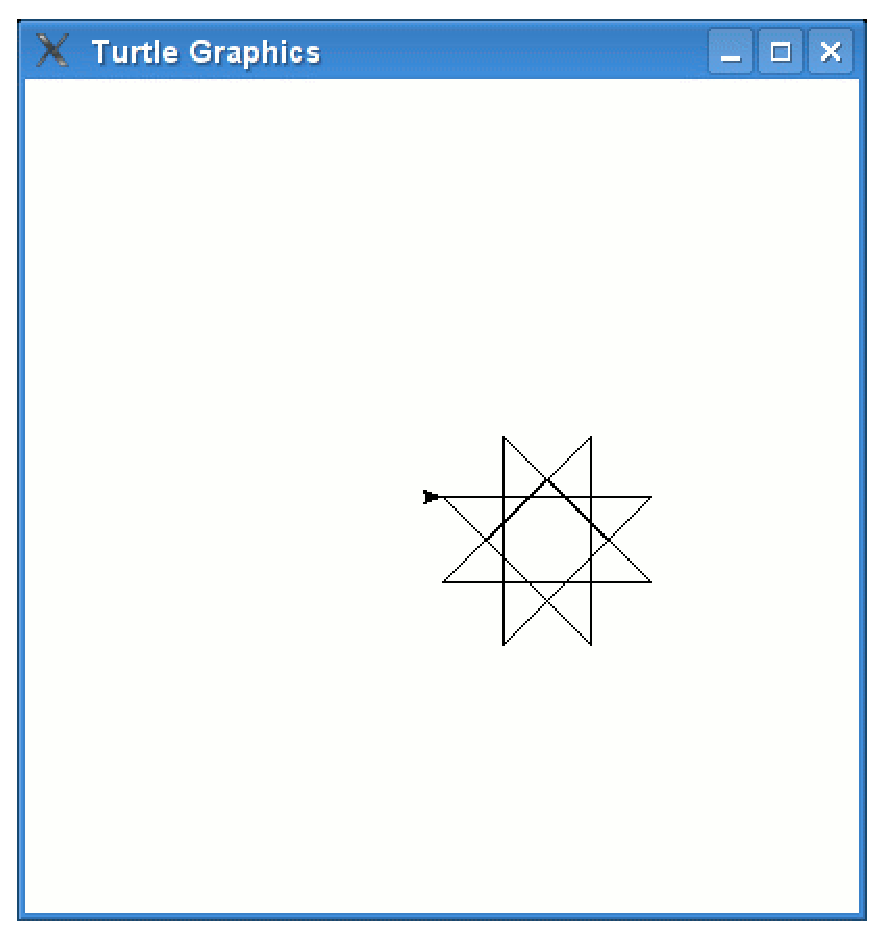
\includegraphics[width=72mm]{figure20.eps}
\end{center}
%\caption{The turtle drawing an 8-point star.}\label{fig20}
\caption{Die Schildkröte zeichnet einen 8-zackigen Stern.}\label{fig20}
\end{figure}

\noindent
%With a different angle (175 degrees), and a longer loop (37 times), we can make a star with even more points (shown in figure~\ref{fig21}):
Mit einem anderen Winkel (175 Grad), und einer längeren Schleife (37 mal), können wir einen Stern mit noch mehr Punkten (wie in Abbildung~\ref{fig21}) zeichnen:

%\begin{Verbatim}[frame=single]
%>>> t.reset()
%>>> for x in range(1,38):
%...     t.forward(100)
%...     t.left(175)
%...
%\end{Verbatim}
\begin{Verbatim}[frame=single]
>>> schildkroete.reset()
>>> for x in range(1,38):
...     schildkroete.forward(100)
...     schildkroete.left(175)
...
\end{Verbatim}

\begin{figure}
\begin{center}
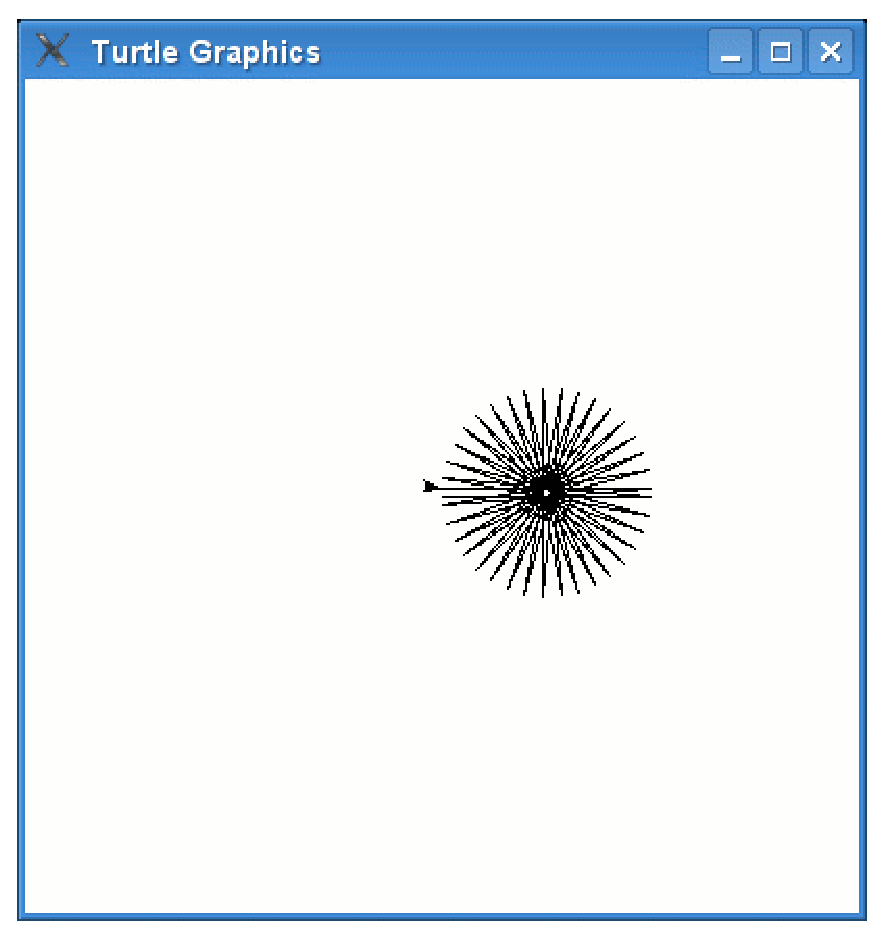
\includegraphics[width=72mm]{figure21.eps}
\end{center}
%\caption{A star with a lot more points.}\label{fig21}
\caption{Ein Stern mit vielen Spitzen.}\label{fig21}
\end{figure}

\noindent
%Or how about the following code, which produces the spiral-like star figure~\ref{fig22}.
Probier mal diesen Code aus, der ein spiralenähnlichen Stern wie in Abbildung~\ref{fig22} erzeugt:

%\begin{Verbatim}[frame=single]
%>>> for x in range(1,20):
%...     t.forward(100)
%...     t.left(95)
%...
%\end{Verbatim}
\begin{Verbatim}[frame=single]
>>> for x in range(1,20):
...     schildkroete.forward(100)
...     schildkroete.left(95)
...
\end{Verbatim}

\begin{figure}
\begin{center}
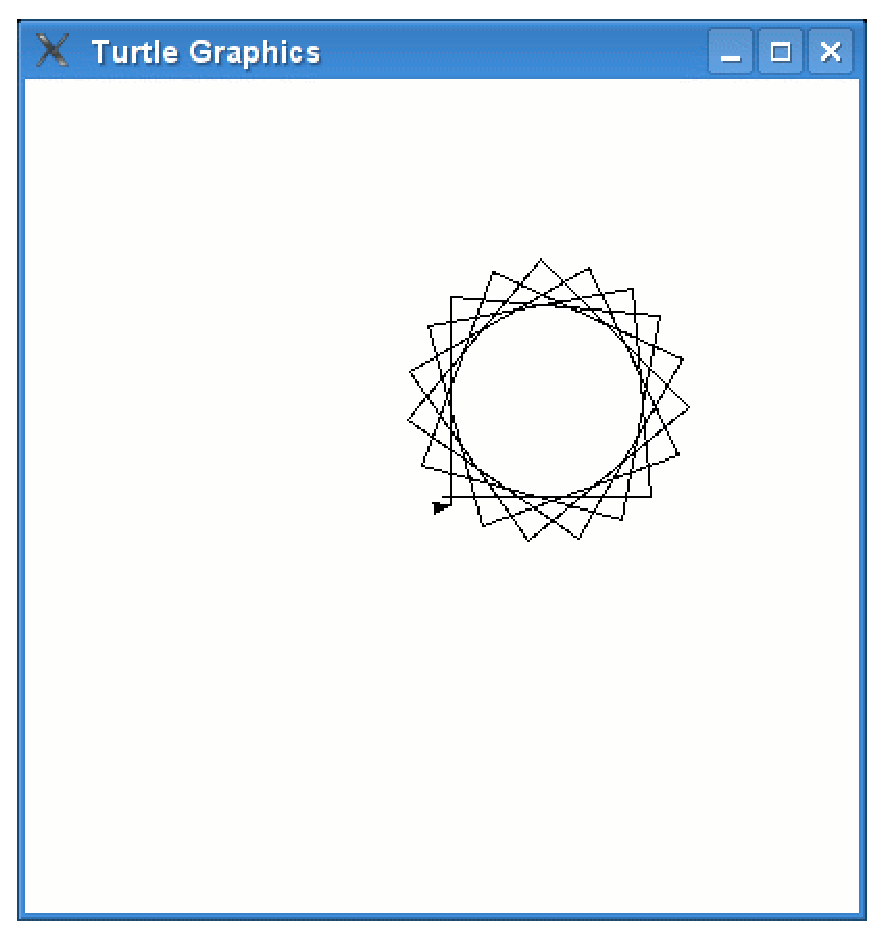
\includegraphics[width=72mm]{figure22.eps}
\end{center}
%\caption{A star with a lot more points.}\label{fig22}
\caption{Ein Stern mit viel mehr Spitzen.}\label{fig22}
\end{figure}

\noindent
%Here's something a bit more complicated:
Und hier etwas komplizierteres:

%\begin{Verbatim}[frame=single]
%>>> t.reset()
%>>> for x in range(1,19):
%...     t.forward(100)
%...     if x % 2 == 0:
%...         t.left(175)
%...     else:
%...         t.left(225)
%...
%\end{Verbatim}
\begin{Verbatim}[frame=single]
>>> schildkroete.reset()
>>> for x in range(1,19):
...     schildkroete.forward(100)
...     if x % 2 == 0:
...         schildkroete.left(175)
...     else:
...         schildkroete.left(225)
...
\end{Verbatim}


%In the above code, we check to see if the variable \code{x} contains an even number.  To do this we use what is called a modulo operator (\%)\index{modulo operator}, in the expression: \code{x \% 2 == 0}.
Im obigen Code wird überprüft, ob \code{x} eine gerade Zahl enthält. Dafür verwenden wir den sogenannten modulo Operator (\%)\\ index{Operator!Modulo}, in der Zeile \code{if x \% 2 == 0:}.
\par
%x \% 2 is equal to zero, if the number in variable \code{x} can be divided by two, with nothing left over (no remainder)---if this doesn't make much sense, don't worry too much about it, just remember you can use `\code{x \% 2 == 0}' to check if a number in a variable is an even number.  The result of running this code is the 9-point star in figure~\ref{fig23}.
x \% 2 ist dann Null, wenn die Nummer in der Variable \code{x} durch 2 dividiert werden kann, ohne das ein Rest übrigbleibt---wenn das keinen Sinn macht, mach dir keine Sorgen, Merke dir nur, dass du `\code{x \% 2 == 0}' dafür verwenden kannst, ob eine Nummer gerade ist. Wenn du den Code ausführst wirst du den 9-zackigen Stern von Abbildung~\ref{fig23} sehen.

\begin{figure}
\begin{center}
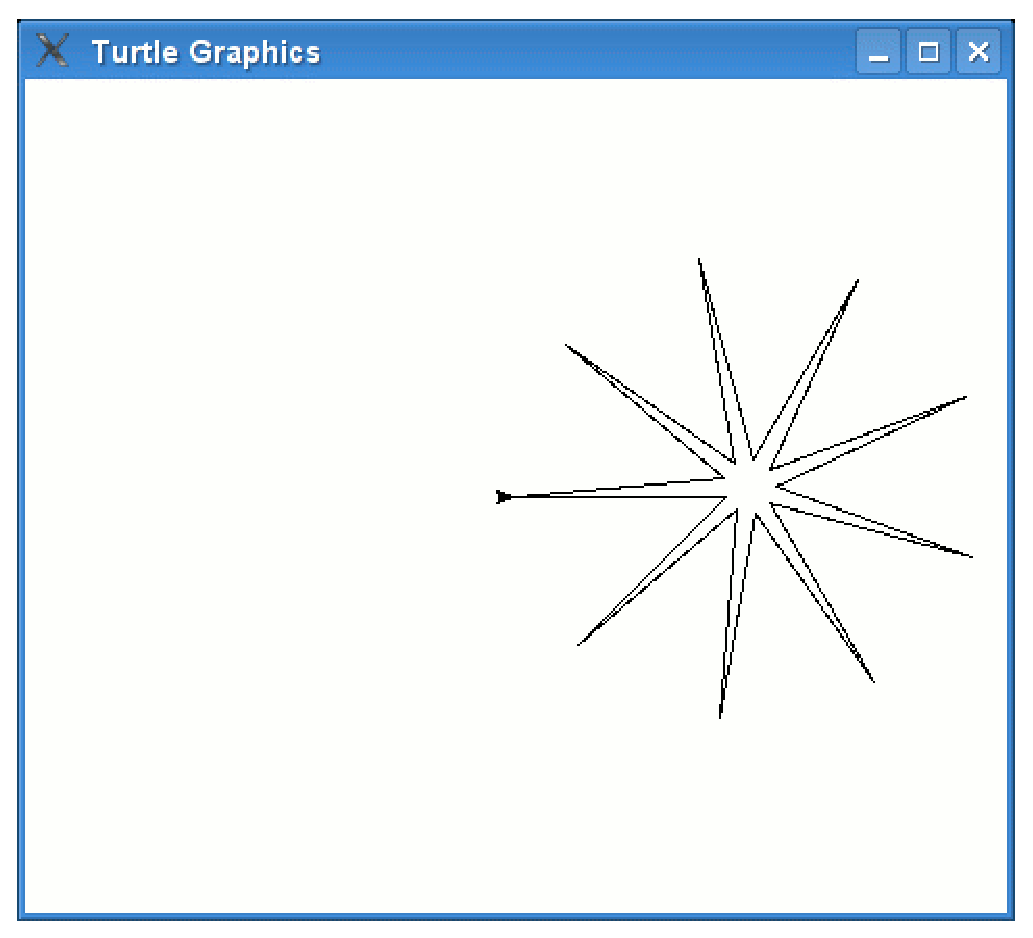
\includegraphics[width=84mm]{figure23.eps}
\end{center}
%\caption{A 9-point star.}\label{fig23}
\caption{Ein 9-zackiger Stern}\label{fig23}
\end{figure}

%You don't have to just draw stars and simple geometric shapes, using a combination of the functions calls, your turtle can draw many different things.  For example:
Du musst nicht immer nur Sterne und einfache Formen zeichnen. Deine Schildkröte kann auch ganz andere Dinge zeichnen. Zum Beispiel:

%\begin{Verbatim}[frame=single]
%t.color(1,0,0)
%t.begin_fill()
%t.forward(100)
%t.left(90)
%t.forward(20)
%t.left(90)
%t.forward(20)
%t.right(90)
%t.forward(20)
%t.left(90)
%t.forward(60)
%t.left(90)
%t.forward(20)
%t.right(90)
%t.forward(20)
%t.left(90)
%t.forward(20)
%t.end_fill()
%t.color(0,0,0)
%t.up()
%t.forward(10)
%t.down()
%t.begin_fill()
%t.circle(10)
%t.end_fill()
%t.setheading(0)
%t.up()
%t.forward(90)
%t.right(90)
%t.forward(10)
%t.setheading(0)
%t.begin_fill()
%t.down()
%t.circle(10)
%t.end_fill()
%\end{Verbatim}
\begin{Verbatim}[frame=single]
schildkroete.color(1,0,0)
schildkroete.begin_fill()
schildkroete.forward(100)
schildkroete.left(90)
schildkroete.forward(20)
schildkroete.left(90)
schildkroete.forward(20)
schildkroete.right(90)
schildkroete.forward(20)
schildkroete.left(90)
schildkroete.forward(60)
schildkroete.left(90)
schildkroete.forward(20)
schildkroete.right(90)
schildkroete.forward(20)
schildkroete.left(90)
schildkroete.forward(20)
schildkroete.end_fill()
schildkroete.color(0,0,0)
schildkroete.up()
schildkroete.forward(10)
schildkroete.down()
schildkroete.begin_fill()
schildkroete.circle(10)
schildkroete.end_fill()
schildkroete.setheading(0)
schildkroete.up()
schildkroete.forward(90)
schildkroete.right(90)
schildkroete.forward(10)
schildkroete.setheading(0)
schildkroete.begin_fill()
schildkroete.down()
schildkroete.circle(10)
schildkroete.end_fill()
\end{Verbatim}

\noindent
%Which is a long, long, long, drawn-out way to draw the rather ugly and primitive-looking car in figure~\ref{fig24}. But it does demonstrate a couple of other turtle functions:  \code{color}, to change the colour of the pen being used by the turtle; \code{fill}, which fills in an area of the canvas; and \code{circle}, to draw a circle of a particular size.
Was eine langsame Methode ist, ein ziemlich einfach ausschauendes Auto zu zeichnen (siehe Abbildung~\ref{fig24}. Aber es zeigt einige neue Funktionen, die die Schildkröte beherscht: \code{color}, um die Farbe des Zeichenstifts zu ändern, \code{fill} um einen Bereich mit Farbe zu füllen und \code{circle}, um einen Kreis mit einer bestimmten Größe zu zeichnen.

\begin{figure}
\begin{center}
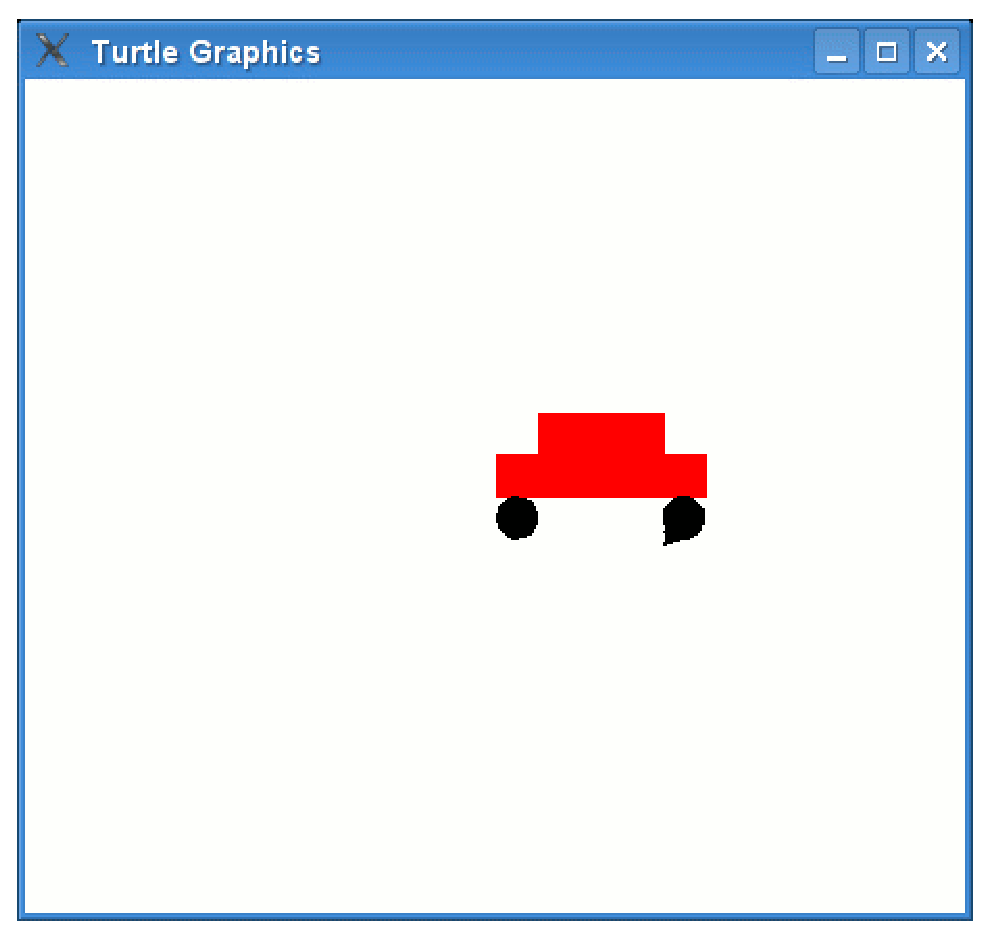
\includegraphics[width=80mm]{figure24.eps}
\end{center}
%\caption{The turtle is terrible at drawing cars!}\label{fig24}
\caption{Die Schildkröte muss noch üben um schöne Autos zu zeichnen!}\label{fig24}
\end{figure}

%\section{Colouring in}
\section{Mit Farben füllen}
%The \code{color}\index{turtle!color} function takes 3 parameters. The first parameter is a value for red, the second is a value for green, and the last is a value for blue.
Die \code{color}\index{Schildkröte!Farbe} Funktion nimmt 3 Parameter.
\par
%\emph{Why red, green and blue?}
\emph{Warum rot, grün und blau?}
\par
%If you've ever played around with different colours of paint, you'll already know part of the answer to that question.  When you mix two different paint colours, you get another colour\footnote{Actually, the three \textbf{primary} paint colours are red, yellow and blue, and not the red/green/blue (RGB) on a computer.}.  When you mix blue and red together, you get purple$\ldots$ and when you mix too many colours together, you usually get a muddy brown. On a computer you can mix colours together in a similar fashion---put red and green together to get yellow---except with a computer, we are combining colours of light, not colours of paint.
Wenn du schon mal mit verschiedenen Farben des Malkastens herumgespielt hast, dann kennst du die Antwort schon fast. Wenn du zwei verschiedene Farben mischt, bekommst du eine andere Farbe\footnote{Eigentlich sind die 3 \textbf{Grundfarben} beim Malen rot, gelb und blau, und nicht rot, grün und blau (RGB) wie auf dem Computer. Malen vs. Computer ist der Unterschied subtraktive vs. additive Farbmischung} Wenn du beim Malen die Blau und Rot zusammenmischt bekommst du ein Lila$\ldots$ und wenn du zu viele Farben mischt erhältst du für gewöhnlich einen bräunlichen Ton. Auf dem Computer kannst du Farben in einer ähnlichen Weise mischen---bringe rot und grün zusammen und es kommt gelb raus---beim Computer mischt du aber Lichter und beim Malen Farben.

%Even though we're not using paint, for a moment, think about 3 large pots of paint.  One red, one green, and one blue.  Each pot is full, so we'll say that a full pot of paint has a value of 1 (or 100\%).  We then pour all of the red paint (100\%) into a vat, followed by all of the green paint (again 100\%).  After a bit of mixing, we get a yellow colour.  Let's draw a yellow circle using turtle:
Denke dir drei große Farbtöpfe mit Farbe. Ein roter, ein grüner und ein blauer Farbtopf. Jede Topf ist voll und wir sagen sie hat den Wert 1 (oder 100\%). Dann leeren wir den ganzen roten (100\%) und grünen (100\%) Topf in einen leeren Behälter und mischen. Nach etwas rühren bekommen wir eine gelbe Farbe. Lass uns nun einen gelben Kreis mit unserer Schildkröte zeichnen:

%\begin{Verbatim}[frame=single]
%>>> t.color(1,1,0)
%>>> t.begin_fill()
%>>> t.circle(50)
%>>> t.end_fill()
%\end{Verbatim}
\begin{Verbatim}[frame=single]
>>> schildkroete.color(1,1,0)
>>> schildkroete.begin_fill()
>>> schildkroete.circle(50)
>>> schildkroete.end_fill()
\end{Verbatim}

%So in the above example, we call the color function with 100\% for red, 100\% for green and 0\% for blue (in other words, 1, 1, and 0).  To make it easier to experiment with different colours, let's turn that into a function:
Im obigen Beispiel rufen wir die \code{color} Funktion mit 100\% für rot, 100\% für grün und 0\% für blau auf (oder in anderen Worten 1, 1, 0). Um das experimentieren mit anderen Farben einfacher zu machen, packen wir das alles in eine Funktion:

%\begin{Verbatim}[frame=single]
%>>> def mycircle(red, green, blue):
%...     t.color(red, green, blue)
%...     t.begin_fill()
%...     t.circle(50)
%...     t.end_fill()
%...
%\end{Verbatim}
\begin{Verbatim}[frame=single]
>>> def mein_kreis(rot, gruen, blau):
...     schildkroete.color(rot, gruen, blau)
...     schildkroete.begin_fill()
...     schildkroete.circle(50)
...     schildkroete.end_fill()
...
\end{Verbatim}

\noindent
%We can draw a bright green circle, by using all of the green paint (1 or 100\%):
Jetzt können wir einen hellen grünen Kreis zeichnen mit der ganzen grünen Farbe (1 oder 100\%) zeichnen:

%\begin{Verbatim}[frame=single]
%>>> mycircle(0, 1, 0)
%\end{Verbatim}
\begin{Verbatim}[frame=single]
>>> mein_kreis(0, 1, 0)
\end{Verbatim}

\noindent
%And we can draw a darker green circle, by using only half the green paint (0.5 or 50\%):
Und einen Kreis mit dunklerem Grün können wir zeichnen indem wir nur das halbe grün (0.5 oder 50\%) verwenden.

%\begin{Verbatim}[frame=single]
%>>> mycircle(0, 0.5, 0)
%\end{Verbatim}
\begin{Verbatim}[frame=single]
>>> mein_kreis(0, 0.5, 0)
\end{Verbatim}

%Here's where thinking about paint doesn't make much sense any more.  In the real world, if you've got a pot of green paint, it doesn't matter how much you use, it's still going to look the same.  With colours on a computer, because we're playing with light, using less of that colour generally results in a darker shade.  It's the same as if you shine a torch at night, you get a yellowish light---when the batteries start to run out and the light begins to fade, the yellow colour gets darker and darker.  Just to see for yourself, try drawing a circle with full red and half red (1 and 0.5), and full blue and half blue.
Hier macht die Analogie mit dem Farbtopf nicht mehr viel Sinn. In der echten Welt ist es egal wieviel man von einer Farbe nimmt, sie schaut immer gleich aus. Da am Computer die Farben aus Licht bestehen macht es einen Unterschied. Weniger Licht (weniger Farbe) erscheint dunkler. Das ist das gleiche mit einer Taschenlampe in der Nacht. Wenn die Batterien immer schwächer werden, wird das Licht immer dunkler. Probiere es am Computer selber aus indem du einen roten Kreis (1, 0, 0) und einen `halbroten' (0.5, 0, 0) und einen blauen und `halbblauen' Kreis zeichnest.

%\begin{Verbatim}[frame=single]
%>>> mycircle(1, 0, 0)
%>>> mycircle(0.5, 0, 0)

%>>> mycircle(0, 0, 1)
%>>> mycircle(0, 0, 0.5)
%\end{Verbatim}
\begin{Verbatim}[frame=single]
>>> mein_kreis(1, 0, 0)
>>> mein_kreis(0.5, 0, 0)

>>> mein_kreis(0, 0, 1)
>>> mein_kreis(0, 0, 0.5)
\end{Verbatim}

\noindent
%Different combinations of red, green and blue will produce a huge variety of colours.  You can get a gold colour by using 100\% of red, 85\% of green and no blue:
Verschiedenen Kombinationen von rot, grün und blau erzeugen alle möglichen Farben. Eine goldene Farbe gibt es wenn du 100\% rot, 85\% grün und kein blau verwendest:

%\begin{Verbatim}[frame=single]
%>>> mycircle(1, 0.85, 0)
%\end{Verbatim}
\begin{Verbatim}[frame=single]
>>> mein_kreis(1, 0.85, 0)
\end{Verbatim}

\noindent
%A light pink colour can be achieved by combining 100\% red, 70\% green and 75\% blue:
Eine rosarote Farbe erreichst du mit 100\% rot, 70\% grün und 75\% blau:

%\begin{Verbatim}[frame=single]
%>>> mycircle(1, 0.70,0.75)
%\end{Verbatim}
\begin{Verbatim}[frame=single]
>>> mein_kreis(1, 0.70,0.75)
\end{Verbatim}

\noindent
%And you get orange by combining 100\% red and 65\% green; and brown by combining 60\% red, 30\% green and 15\% blue:
Orange wird die Mischung aus 100\% rot und 65\% grün; Braun ist 60\% rot, 30\% grün und 15\% blau:

%\begin{Verbatim}[frame=single]
%>>> mycircle(1, 0.65, 0)
%>>> mycircle(0.6, 0.3, 0.15)
%\end{Verbatim}
\begin{Verbatim}[frame=single]
>>> mein_kreis(1, 0.65, 0)
>>> mein_kreis(0.6, 0.3, 0.15)
\end{Verbatim}

\noindent
%Don't forget, you can clear the canvas by using \code{t.clear()}.
Die Leinwand kannst du wieder mit \code{schildkroete.clear()} löschen.

%\section{Darkness}\index{turtle!color!black}
\section{Die Dunkelheit}\index{Schildkröte!Farbe!schwarz}

%Here's a question for you:  What happens when you turn all the lights off at night? Everything goes black.
Eine kleine Frage für dich: Was passiert, wenn du in der Nacht alle Lampen ausschaltest? Alles wird schwarz.
\par
%The same thing happens with colours on a computer.  No light equals no colour.  So a circle with 0 for red, 0 for green and 0 for blue:
Das gleiche passiert mit den Farben am Computer. Kein Licht bedeutet keine Farbe. Ein Kreis mit 0 für rot, 0 für grün und 0 für blau schaut so aus:

%\begin{Verbatim}[frame=single]
%>>> mycircle(0, 0, 0)
%\end{Verbatim}
\begin{Verbatim}[frame=single]
>>> mein_kreis(0, 0, 0)
\end{Verbatim}

%Produces the black spot in figure~\ref{fig25}.
Und das ergibt einen dicken schwarzen Punkt (wie in Abbildung~\ref{fig25}.

\begin{figure}
\begin{center}
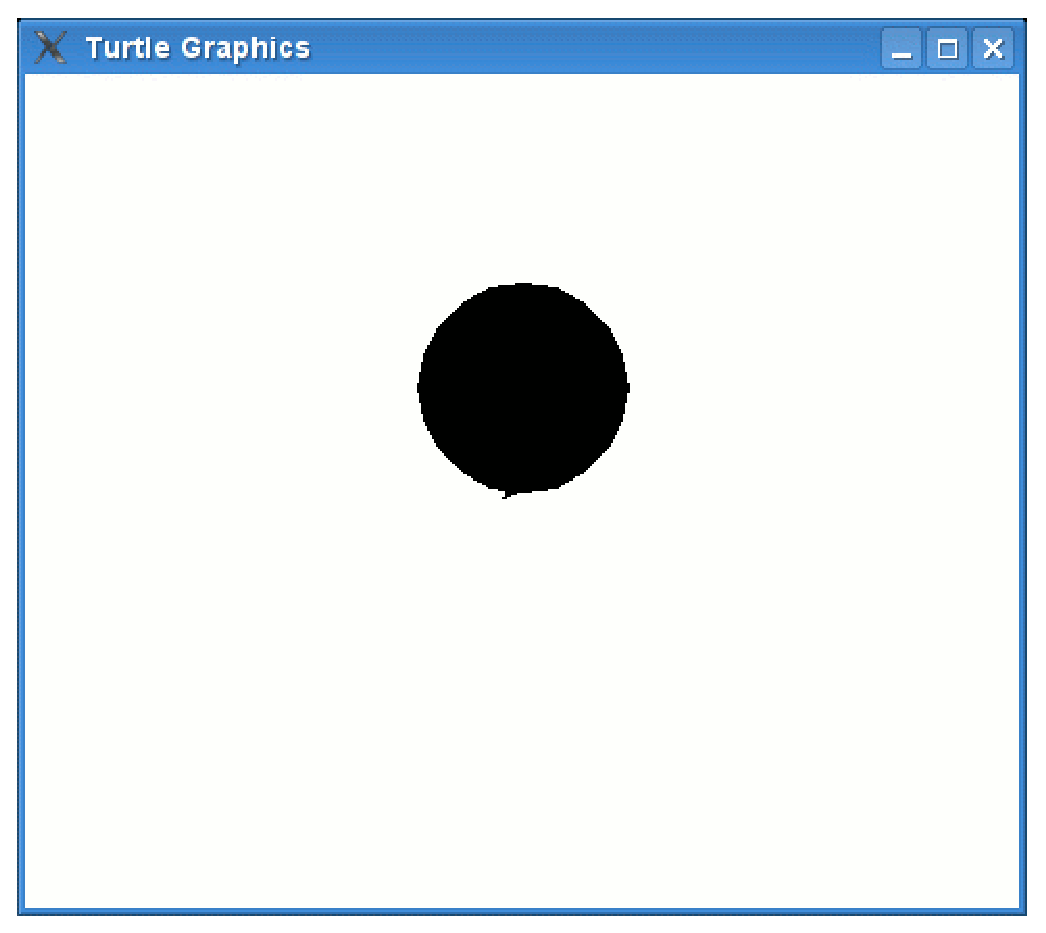
\includegraphics[width=85mm]{figure25.eps}
\end{center}
%\caption{A black hole!}\label{fig25}
\caption{Ein schwarzes Loch!}\label{fig25}
\end{figure}

%The opposite is true; if you use 100\% red, 100\% green and 100\% blue, you get white.  Use the following code and the black circle will be wiped out again:
Und auch das Gegenteil ist wahr; wenn du 100\% für rot, 100\% für grün und 100\% für blau verwendest, bekommst du weiß. Nimm den folgenden Code und der schwarze Kreis wird wieder ausgelöscht:

%\begin{Verbatim}[frame=single]
%>>> mycircle(1,1,1)
%\end{Verbatim}
\begin{Verbatim}[frame=single]
>>> mein_kreis(1,1,1)
\end{Verbatim}

%\section{Filling things}\index{turtle!fill}
\section{Dinge füllen}\index{Schildkröte!mit Farben ausfüllen}

%You've probably figured out by now that the fill function is switched on by passing the parameter `1', then switched off again with `0'. When you switch it off, the function actually fills in the area you've drawn---assuming you've drawn at least part of a shape. So we can easily draw a filled in square by using code we created earlier. First, let's turn it into a function. To draw a square with turtle we do:
Du hast vielleicht herausgefunden, dass durch die Übergabe des Parameters `1' die \code{fill} Funktion eingeschalten wird. Mit dem Parameter `0' wir die Funktion wieder ausgeschalten. Beim ausschalten wird die bisher gezeichnete Form ausgemalt. So können wir einfach aufgefüllte Quadrate zeichnen indem wir den Code von früher verwenden. Um ein Quadrat mit der Schildkröte zu zeichnen gibst du folgendes ein:

%\begin{Verbatim}[frame=single]
%>>> t.forward(50)
%>>> t.left(90)
%>>> t.forward(50)
%>>> t.left(90)
%>>> t.forward(50)
%>>> t.left(90)
%>>> t.forward(50)
%>>> t.left(90)
%\end{Verbatim}
\begin{Verbatim}[frame=single]
>>> schildkroete.forward(50)
>>> schildkroete.left(90)
>>> schildkroete.forward(50)
>>> schildkroete.left(90)
>>> schildkroete.forward(50)
>>> schildkroete.left(90)
>>> schildkroete.forward(50)
>>> schildkroete.left(90)
\end{Verbatim}

%So as a function, we might want to pass the size of the square as a parameter.  This makes the function a little more flexible:
Etwas flexibler wird das ganze, wenn wir eine Funktion erzeugen und die Größe des Quadrats als Parameter mitgeben:

%\begin{Verbatim}[frame=single]
%>>> def mysquare(size):
%...     t.forward(size)
%...     t.left(90)
%...     t.forward(size)
%...     t.left(90)
%...     t.forward(size)
%...     t.left(90)
%...     t.forward(size)
%...     t.left(90)
%\end{Verbatim}
\begin{Verbatim}[frame=single]
>>> def mein_quadrat(groesse):
...     schildkroete.forward(groesse)
...     schildkroete.left(90)
...     schildkroete.forward(groesse)
...     schildkroete.left(90)
...     schildkroete.forward(groesse)
...     schildkroete.left(90)
...     schildkroete.forward(groesse)
...     schildkroete.left(90)
\end{Verbatim}

\noindent
%We can test our function by calling:
Du kannst die Funktion aufrufen, indem du folgendes eingibst:

%\begin{Verbatim}[frame=single]
%>>> mysquare(50)
%\end{Verbatim}
\begin{Verbatim}[frame=single]
>>> mein_quadrat(50)
\end{Verbatim}

%That's a start, but it's not quite perfect.  If you look at the code above, you'll see a pattern.  We repeat: \code{forward(size)} and \code{left(90)} four times.  That's a waste of typing.  So we can use a for-loop to do it for us (pretty much the same as we did earlier):
Als Anfang schon ganz gut, aber noch nicht perfekt. Wenn du den Code oben anschaust, wirst du ein Muster erkennen. Wir wiederholen: \code{forward(groesse)} und \code{left(90)} vier Mal. Das ist unnötige Tipparbeit. Wie können eine for-Schleife verwenden die uns das erspart:

%\begin{Verbatim}[frame=single]
%>>> def mysquare(size):
%...     for x in range(0,4):
%...         t.forward(size)
%...         t.left(90)
%\end{Verbatim}
\begin{Verbatim}[frame=single]
>>> def mein_quadrat(groesse):
...     for x in range(0,4):
...         schildkroete.forward(groesse)
...         schildkroete.left(90)
\end{Verbatim}

%That's a big improvement on the previous version. You can test the function with different sizes:
Das ist eine große Verbesserung zur vorigen Version. Testen wir die Funktion mit verschiedenen Größen (verschiedenen Parametern):

%\begin{Verbatim}[frame=single]
%>>> t.reset()
%>>> mysquare(25)
%>>> mysquare(50)
%>>> mysquare(75)
%>>> mysquare(100)
%>>> mysquare(125)
%\end{Verbatim}
\begin{Verbatim}[frame=single]
>>> schildkroete.reset()
>>> mein_quadrat(25)
>>> mein_quadrat(50)
>>> mein_quadrat(75)
>>> mein_quadrat(100)
>>> mein_quadrat(125)
\end{Verbatim}

%And the turtle should draw something like figure~\ref{fig26}.
Und unsere Schildkröte wird etwas zeichnen das wie in Abbildung~\ref{fig26} aussieht.

\begin{figure}
\begin{center}
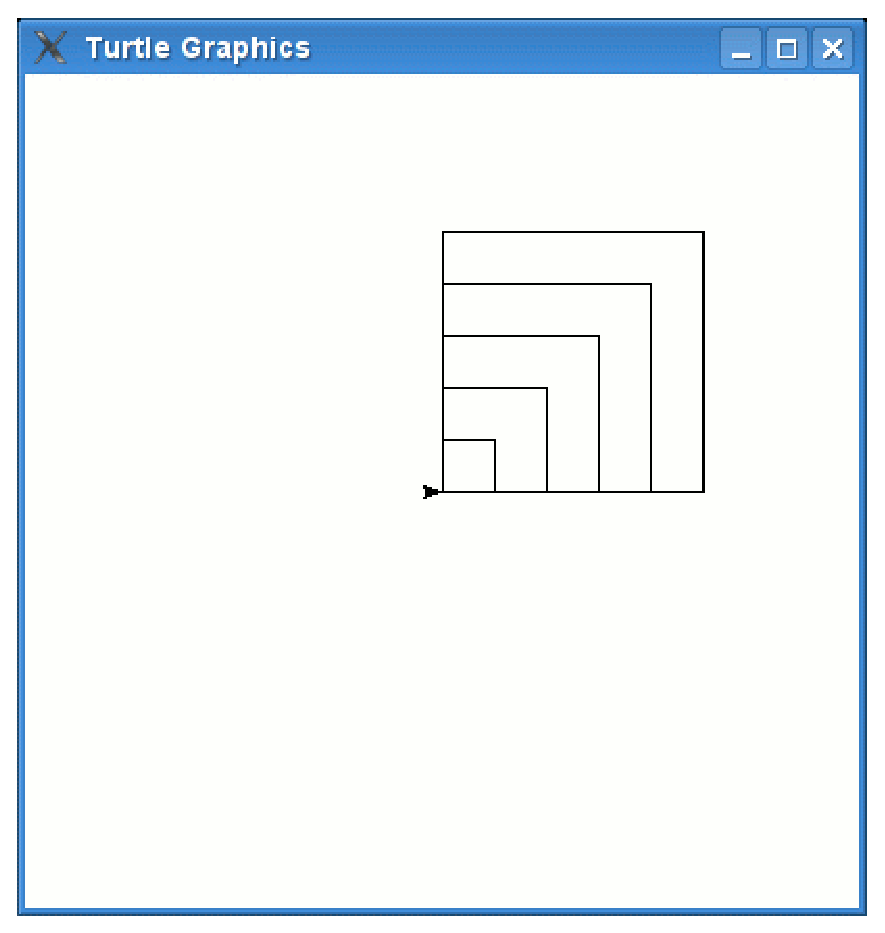
\includegraphics[width=72mm]{figure26.eps}
\end{center}
%\caption{Lots of squares.}\label{fig26}
\caption{Viele Quadrate.}\label{fig26}
\end{figure}

\noindent
%Now we can try a filled square.  First of all, reset the canvas once again:
Jetzt versuchen wir das Quadrat mit Farbe zu füllen. Zuerst löschen wir die Leinwand:

%\begin{Verbatim}[frame=single]
%>>> t.reset()
%\end{Verbatim}
\begin{Verbatim}[frame=single]
>>> schildkroete.reset()
\end{Verbatim}

\noindent
%Then, turn on filling, and call the square function again:
Dann schalten wir `ausfüllen' ein und rufen nochmals die Funktion \code{mein\_quadrat} auf:

%\begin{Verbatim}[frame=single]
%>>> t.begin_fill()
%>>> mysquare(50)
%\end{Verbatim}
\begin{Verbatim}[frame=single]
>>> schildkroete.begin_fill()
>>> mein_quadrat(50)
\end{Verbatim}

\noindent
%You'll still see an empty square until you turn filling off:
Du siehst immer noch das leere Quadrat bis du die Funktion `ausfüllen' wieder ausschaltest.

%\begin{Verbatim}[frame=single]
%>>> t.end_fill()
%\end{Verbatim}
\begin{Verbatim}[frame=single]
>>> schildkroete.end_fill()
\end{Verbatim}

\noindent
%Which produces something like the square in figure~\ref{fig27}.
Und nun erhälts du etwas wie Bild~\ref{fig27}.

\begin{figure}
\begin{center}
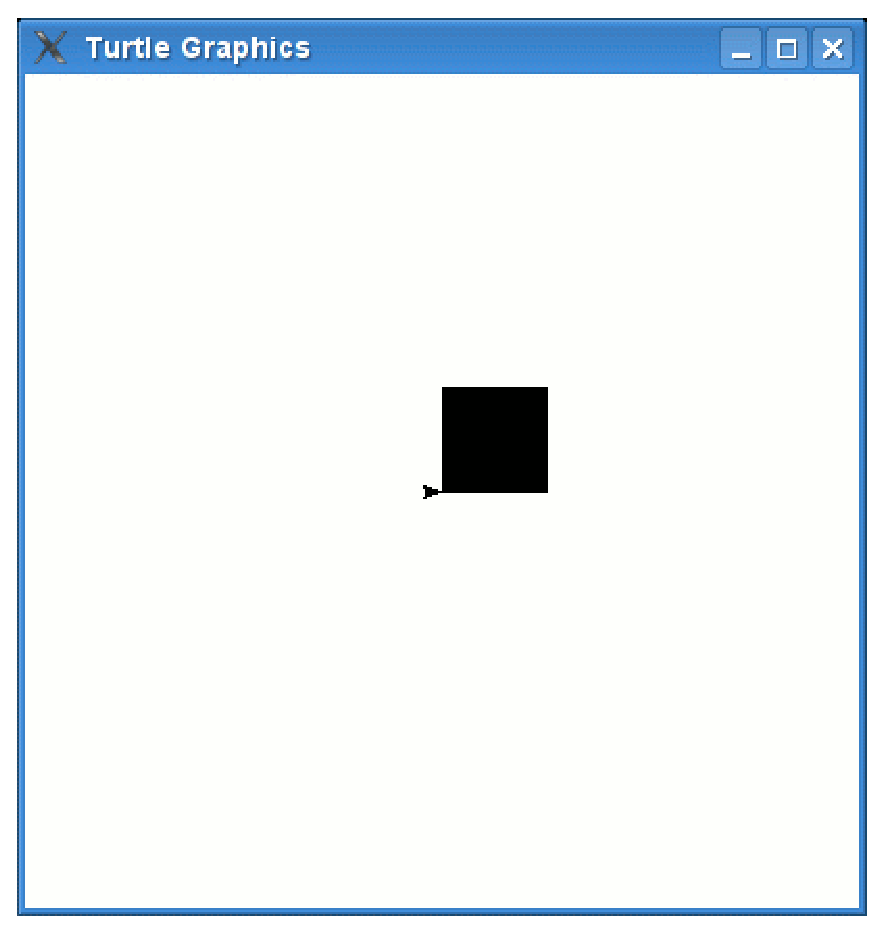
\includegraphics[width=72mm]{figure27.eps}
\end{center}
%\caption{A black square.}\label{fig27}
\caption{Ein schwarzes Quadrat.}\label{fig27}
\end{figure}

%How about changing the function so that we can either draw a filled or an unfilled square? We need another parameter, and slightly more complicated code, to do this:
Sollen wir unsere Funktion ein wenig verändern, damit wir entweder befüllte oder unbefüllte Quadrate zeichen können? Dazu verwenden wir einen zusätzlichen Parameter, um das anzustellen:

%\begin{Verbatim}[frame=single]
%>>> def mysquare(size, filled):
%...    if filled == True:
%...        t.begin_fill()
%...    for x in range(0,4):
%...        t.forward(size)
%...        t.left(90)
%...    if filled == True:
%...        t.end_fill()
%...
%\end{Verbatim}
\begin{Verbatim}[frame=single]
>>> def mein_quadrat(groesse, fuellen):
...    if fuellen == True:
...        schildkroete.begin_fill()
...    for x in range(0,4):
...        schildkroete.forward(groesse)
...        schildkroete.left(90)
...    if fuellen == True:
...        schildkroete.end_fill()
...
\end{Verbatim}

%The first two lines check to see if the value of parameter `filled' is set to True. If it is, then filling is turned on.  We then loop four times to draw the four sides of the rectangle, before checking a second time whether the parameter `filled' is True, and if so, turn filling off once again. You can now draw a filled square by calling:
Die ersten zwei Zeilen überprüfen ob der Parameter `fuellen' auf True gesetzt wurde. Wenn ja wird \code{filling} ein geschalten. Dann wird die Schleife vier mal durchlaufen und danach wieder der Paramter `fuellen' überprüft. Wenn ja, dann wird \code{filling} wieder ausgeschalten. Ein gefülltes Quadrat kann also so gezeichnet werden:

\begin{Verbatim}[frame=single]
>>> mein_quadrat(50, True)
\end{Verbatim}

\noindent
%And an unfilled square by calling:
Und ein leeres Quadrat so:

%\begin{Verbatim}[frame=single]
%>>> mysquare(150, False)
%\end{Verbatim}
\begin{Verbatim}[frame=single]
>>> mein_quadrat(150, False)
\end{Verbatim}

\noindent
%Which causes our turtle to draw the image in figure~\ref{fig28}$\ldots$ $\ldots$which, now that I think about it, looks like a weird square eye.
Als Ergebnis zeichnet die Schildkröte ein Bild wie in Abbildung~\ref{fig28}$\ldots$ $\ldots$ und das schaut ein wenig wie ein seltsames viereckiges Auge aus.

\begin{figure}
\begin{center}
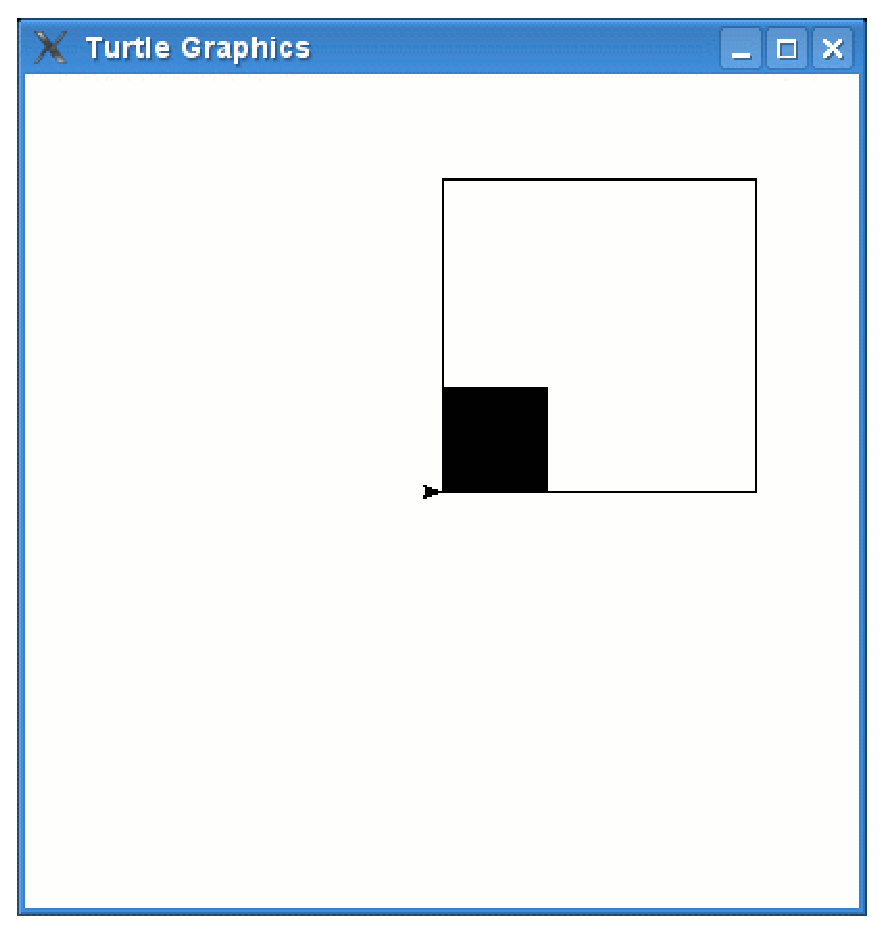
\includegraphics[width=72mm]{figure28.eps}
\end{center}
\caption{A square eye.}\label{fig28}
\end{figure}

%You can draw all sorts of shapes and fill them with colour. Let's turn the star, we drew earlier, into a function. The original code looked like this:
Du kannst alle möglichen Formen zeichnen und sie mit Farbe füllen. Lass uns den Stern vor vorhin in eine Funktion verpacken. Der original Code hat so ausgeshen:

%\begin{Verbatim}[frame=single]
%>>> for x in range(1,19):
%...     t.forward(100)
%...     if x % 2 == 0:
%...         t.left(175)
%...     else:
%...         t.left(225)
%...
%\end{Verbatim}
\begin{Verbatim}[frame=single]
>>> for x in range(1,19):
...     schildkroete.forward(100)
...     if x % 2 == 0:
...         schildkroete.left(175)
...     else:
...         schildkroete.left(225)
...
\end{Verbatim}

%We can use the same if-statements from the mysquare function, and use the size parameter in the \code{forward} function.
Wie können die gleiche if-Bedingung von der \code{mein\_stern} Funktion nehmen und als Parameter die Größe übergeben:

%\begin{Verbatim}[frame=single]
%1.  >>> def mystar(size, filled):
%2.  ...     if filled:
%3.  ...         t.begin_fill()
%4.  ...     for x in range(1,19):
%5.  ...         t.forward(size)
%6.  ...         if x % 2 == 0:
%7.  ...             t.left(175)
%8.  ...         else:
%9.  ...             t.left(225)
%10. ...     if filled:
%11. ...         t.end_fill()
%\end{Verbatim}
\begin{Verbatim}[frame=single]
1.  >>> def mein_stern(groesse, fuellen):
2.  ...     if fuellen:
3.  ...         schildkroete.begin_fill()
4.  ...     for x in range(1,19):
5.  ...         schildkroete.forward(groesse)
6.  ...         if x % 2 == 0:
7.  ...             schildkroete.left(175)
8.  ...         else:
9.  ...             schildkroete.left(225)
10. ...     if fuellen:
11. ...         schildkroete.end_fill()
\end{Verbatim}

%In lines 2 and 3, we switch filling on, depending upon the value of the parameter \code{filled} (turn filling on, if the parameter is set to True, turn it off, if the parameter is set to False).  We do the reverse in lines 10 and 11 (switch filling back off again).  The other difference about this function is that we pass the size of the star in the parameter \code{size}, and use this value in line 5.
In Zeile 2 und 3 wird abhängig vom Parameter \code{fuellen} die Funktion \code{begin\_fill()} ausgeführt oder nicht (bei `True' ist es an, bei `False' ist es aus). Das verkehrte machen wir bei Zeile 10 und 11. Zusätzlich übergeben wir die Größe als Parameter und verwenden sie in Zeile 5.
\par
%Now let's set the colour to gold (you might remember that gold can be made by using 100\% of red, 85\% of green and no blue), and then call the function:
Lass uns die Farbe nun auf Gold (besteht aus 100\% rot, 85\% grün und ohne blau) setzen und die Funktion nochmals aufrufen.

%\begin{Verbatim}[frame=single]
%>>> t.color(1, 0.85, 0)
%>>> mystar(120, True)
%\end{Verbatim}
\begin{Verbatim}[frame=single]
>>> schildkroete.color(1, 0.85, 0)
>>> mein_stern(120, True)
\end{Verbatim}

\noindent
%The turtle should draw the gold star in figure~\ref{fig29}. We can add an outline for the star, by changing the colour again (this time to black) and redrawing the star with filling turned off
Die Schildkröte sollte nun den goldenen Stern in figure~\ref{fig29} zeichnen. Für die schwarze Umrandung können wir die Farbe nochmals ändern (diesmal auf schwarz) und den Stern nochmals ohne zeichnen ohne ihn mit schwarz auszufüllen.

\begin{figure}
\begin{center}
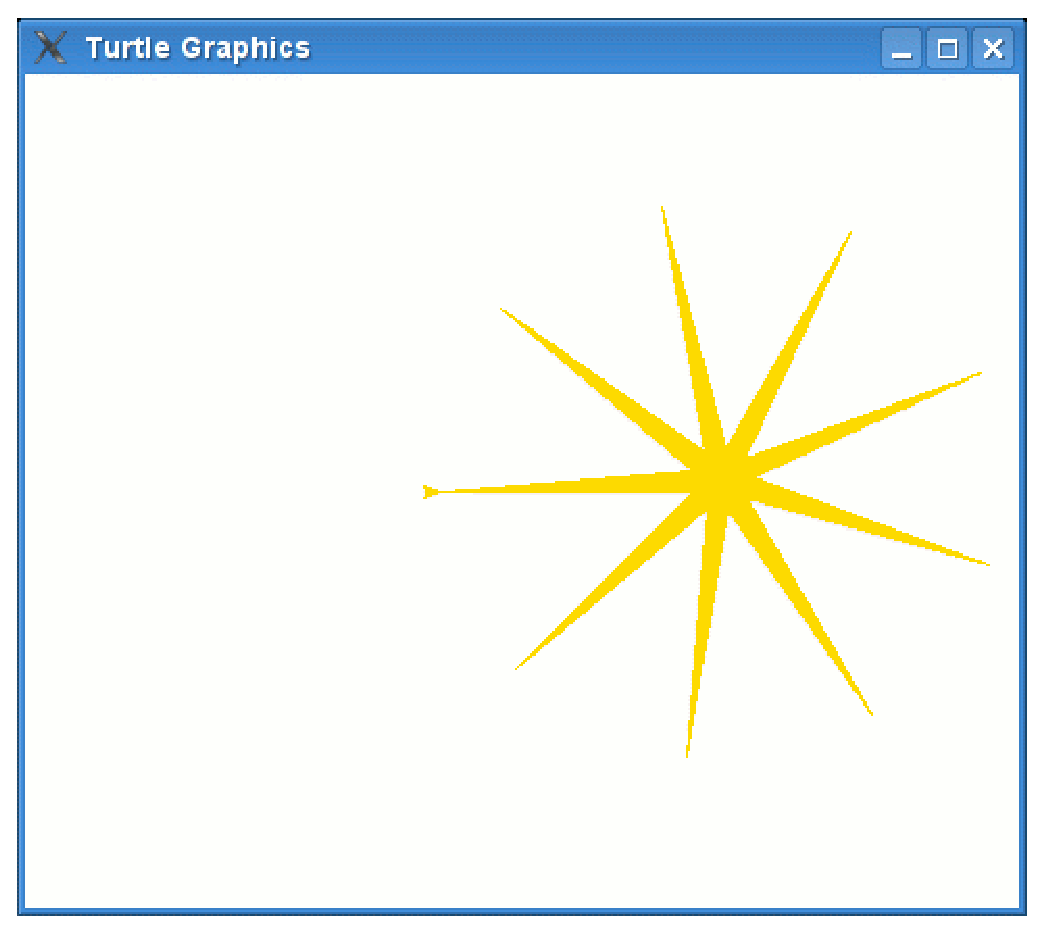
\includegraphics[width=85mm]{figure29.eps}
\end{center}
%\caption{A gold star.}\label{fig29}
\caption{Ein goldener stern.}\label{fig29}
\end{figure}

%\begin{Verbatim}[frame=single]
%>>> t.color(0,0,0)
%>>> mystar(120, False)
%\end{Verbatim}
\begin{Verbatim}[frame=single]
>>> schildkroete.color(0,0,0)
>>> mein_stern(120, False)
\end{Verbatim}

\noindent
%Thus the star now looks like figure~\ref{fig30}.
Und so schaut der Stern nun aus wie Abbildung~\ref{fig30}.

\begin{figure}
\begin{center}
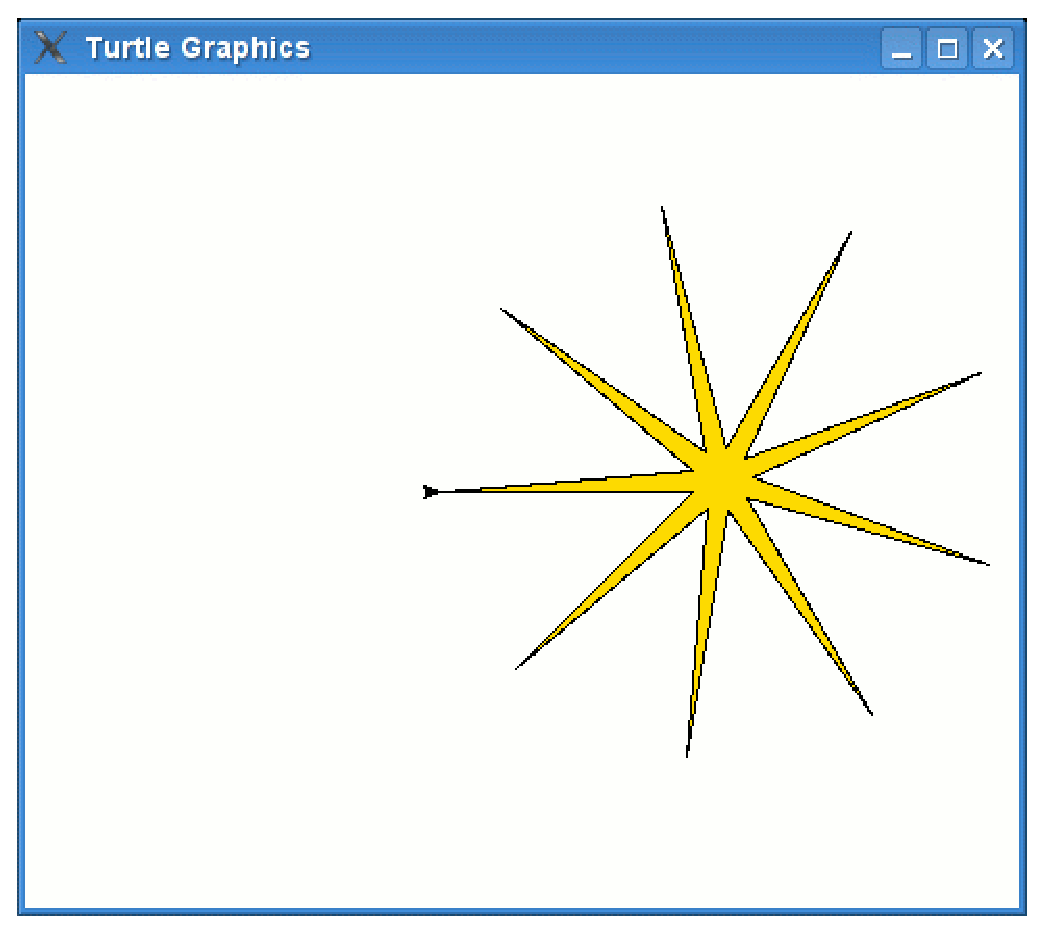
\includegraphics[width=85mm]{figure30.eps}
\end{center}
%\caption{A star with an outline.}\label{fig30}
\caption{Ein Stern mit Umriß.}\label{fig30}
\end{figure}

%\section{Things to try}
\section{Probiere es aus}

%\emph{In this chapter we learned about the turtle module, using it to draw a few basic geometric shapes. We used functions in order to re-use some of our code, to make it easier to draw shapes with different colours.}
\emph{In diesem Kapitel haben wir mehr über das \code{turtle} Modul gelern und es verwendet um geometrische Formen zu zeichnen. Funktionen wurden verwendet um Code wieder zu verwenden und es einfacher zu machen verschiedene Formen zu zeichnen und zu füllen.}

%\subsection*{Exercise 1}
\subsection*{Übung 1}
%We've drawn stars, squares and rectangles.  How about an octagon?  An octagon is an 8 sided shape.
Wir haben Sterne, Quadrate und Rechtecke gezeichnet. Wie schaut es mit einem Achteck  aus? Ein Achteck ist zum Beispiel die Stopptafel, die du oft auf Kreuzungen sehen kannst.
%(Hint: try turning 45 degrees).
(Tipp: versuche mit 45 Grad zu zeichnen).

%\subsection*{Exercise 2}
\subsection*{Übung 2}
%Now convert the octagon drawing code into a function which will fill it with a colour.
Verpacke den Code in eine Funktion und fülle das Achteck mit einer Farbe.

\newpage
